% Two-page A4 LANDSCAPE summary. Page 1 = overview, Page 2 = figure appendix.
\documentclass[a4paper,landscape,10pt]{extarticle}
\usepackage[margin=9mm]{geometry}
\usepackage{graphicx,amsmath,xcolor}
\usepackage{helvet}\renewcommand{\familydefault}{\sfdefault}
\usepackage[T1]{fontenc}
\usepackage{enumitem}\setlist{nosep,leftmargin=3.6mm}
\pagestyle{empty}\setlength{\parindent}{0pt}
\newcommand{\sechead}[1]{\vspace{0.8mm}{\bfseries #1}\\[-2.3mm]\rule{\linewidth}{0.5pt}\\[0.9mm]}
\newcommand{\num}[1]{\textbf{#1}}
\newcommand{\why}[1]{{\itshape\mdseries #1}}
\newcommand{\appfig}[2]{\begin{minipage}[t]{0.325\linewidth}\centering%
  \includegraphics[width=\linewidth,height=3.7cm,keepaspectratio]{../outputs/#1}\\[0.4mm]%
  {\footnotesize #2}\end{minipage}}
\begin{document}
% ===================== PAGE 1 =====================
{\centering
{\LARGE\bfseries Path-ILC with a learned correction layer for high-accuracy industrial robots}\\[1mm]
{\small A flexible-joint KUKA iiwa14 that self-learns its drivetrain error from joint-side encoders, then \emph{generalizes} the correction with a small neural-network layer}\\[1mm]
{\small\textbf{Pravin Oli} \;$\cdot$\; IFROS (Universitat de Girona, Spain \;$\cdot$\; E\"otv\"os Lor\'and University, Hungary) \;$\cdot$\; \texttt{pravin.oli.08@gmail.com}}\\[1mm]}
\rule{\linewidth}{1pt}\\[1.5mm]
\begin{minipage}[t]{0.355\linewidth}
\sechead{Background \& motivation}
Industrial robots are accurate \emph{relative} to themselves but their
\emph{absolute} accuracy is limited by unmodeled \textbf{drivetrain error}:
joint elasticity, gear/cycloidal transmission error, friction, backlash and
thermal drift. Schwegel \& Kugi (ICRA 2024) cancel this with a
\textbf{path-parameter ILC} but need an external \textbf{laser tracker} to learn,
and list open problems: speed variation, \textbf{contact}, a \textbf{model-based
learning filter}, and \textbf{generalizing} the correction to \textbf{new paths}.
\sechead{The robot-arm model I assume}
Each axis $=$ a \textbf{two-mass flexible joint}: motor inertia $J_m$ and link
inertia $J_\ell$ joined by a torsional \textbf{spring $K$ + damper $d$}. The
controller plans on the \emph{rigid} model; the plant deflects, so
$\Delta=\theta_m-\theta_\ell$ is a real, pose/load-dependent transmission error.
\begin{itemize}
\item $K\!\approx$18000$\to$3000\,Nm/rad, $d\!\approx$50$\to$8 (root$\to$wrist)
\item $f_n\!\approx$10--195\,Hz, $\zeta\!\approx$0.1--1.6
\item Gear TE 0.3--0.8\,mrad, 13--37 cyc/rev; backlash 0.5--1.2\,mrad
\item Stribeck $F_s/F_c{=}1.7$; thermal $k_T$ 3--6\,mrad/$T$; 19-bit encoder
\end{itemize}
\sechead{Method}
\begin{center}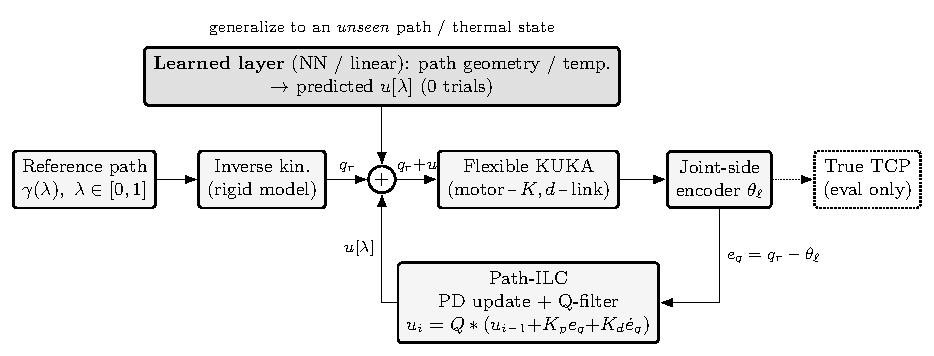
\includegraphics[width=\linewidth]{method_loop.pdf}\end{center}
{\footnotesize The \textbf{path-ILC} learns a table $u[\lambda]$ indexed by the path
parameter $\lambda$ (not time) with a PD update + Gaussian \textbf{Q-filter};
$\lambda$-indexing transfers across speeds. A small \textbf{neural-network layer} predicts
$u[\lambda]$ for an \emph{unseen} path / thermal state with \textbf{zero trials}.}
\end{minipage}\hfill
\begin{minipage}[t]{0.625\linewidth}
\vspace{0pt}
\begin{center}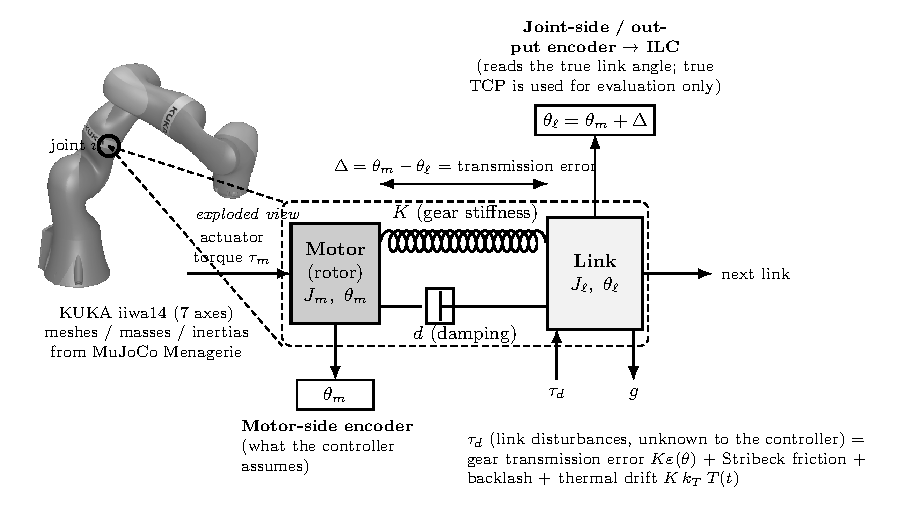
\includegraphics[width=0.84\linewidth]{model_schematic.pdf}\\[0.4mm]
{\footnotesize\textbf{Fig.\,1.}~Drivetrain model. One axis of the real iiwa14 is exploded into motor $J_m$ -- spring $K$/damper $d$ -- link $J_\ell$, with the link disturbance torque $\tau_d$ and the two encoders. The \textbf{joint-side (output) encoder} feeds the ILC; the true TCP is evaluation only.}
\end{center}
\vspace{1mm}
\sechead{Results \,{\normalfont\footnotesize(Cartesian RMS at the tool tip; simulation, seeded/reproducible)}}
\begin{minipage}[t]{0.325\linewidth}\centering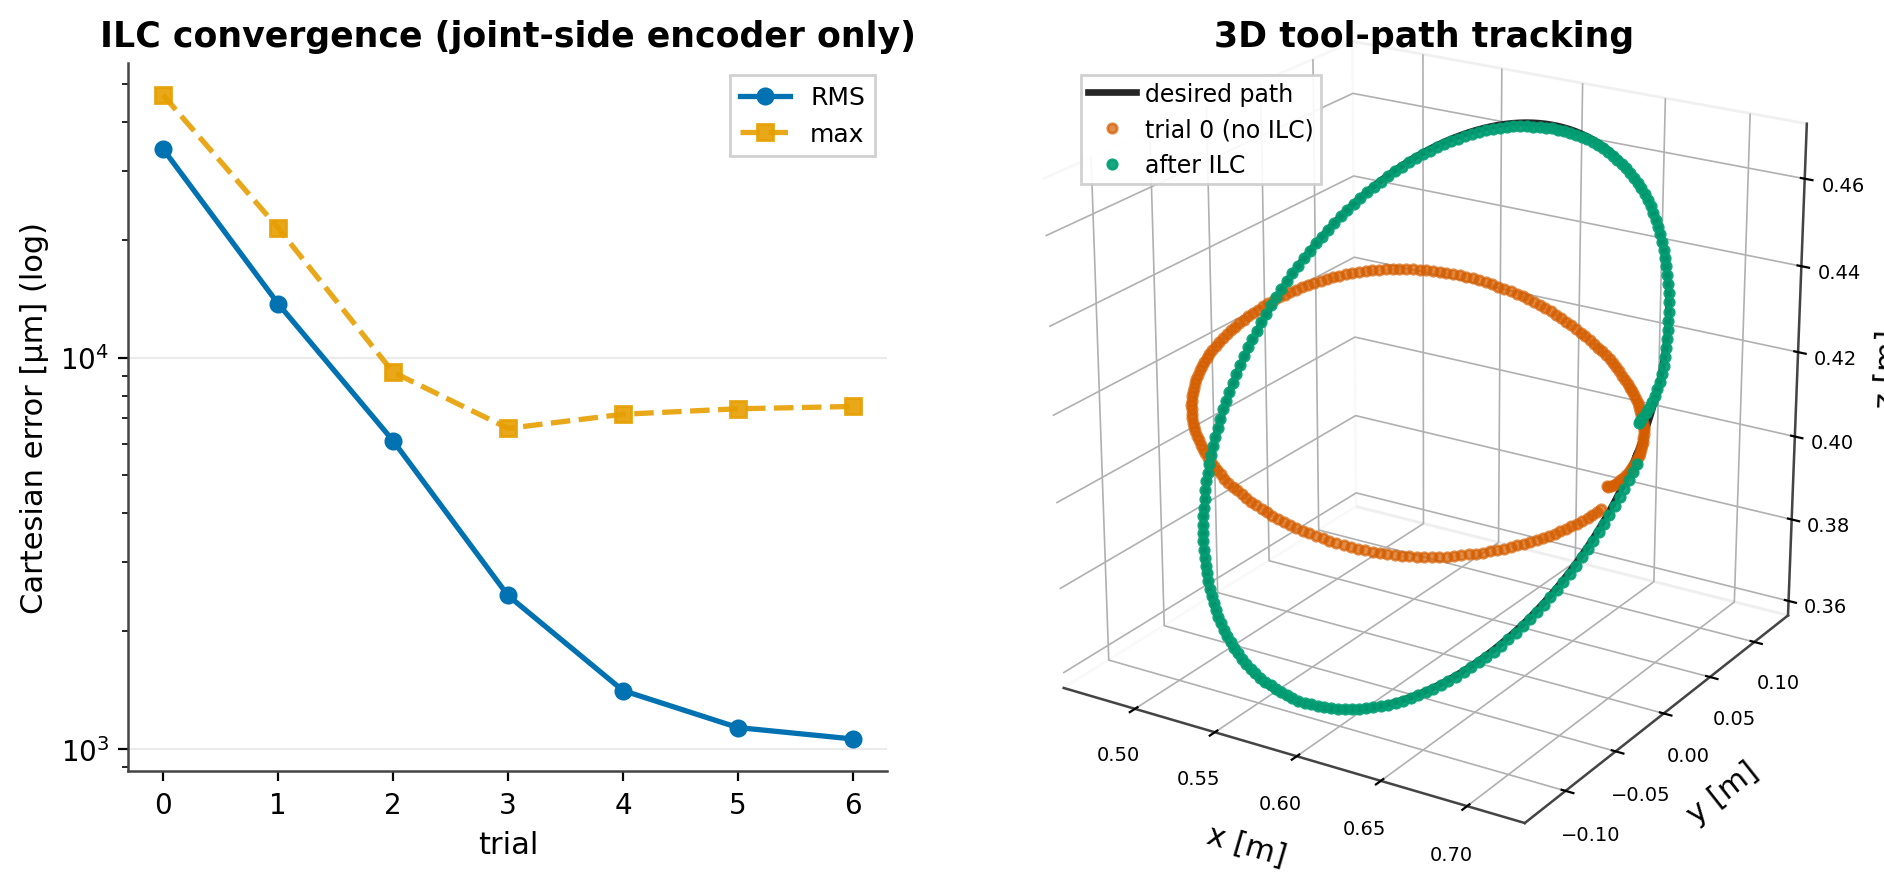
\includegraphics[width=\linewidth]{../outputs/kuka_convergence.png}\\[0.3mm]
{\footnotesize\textbf{Convergence} (encoder only): \num{34156$\to$1061\,$\mu$m, $\sim$32$\times$}\\\why{self-learned without a laser tracker}}\end{minipage}\hfill
\begin{minipage}[t]{0.325\linewidth}\centering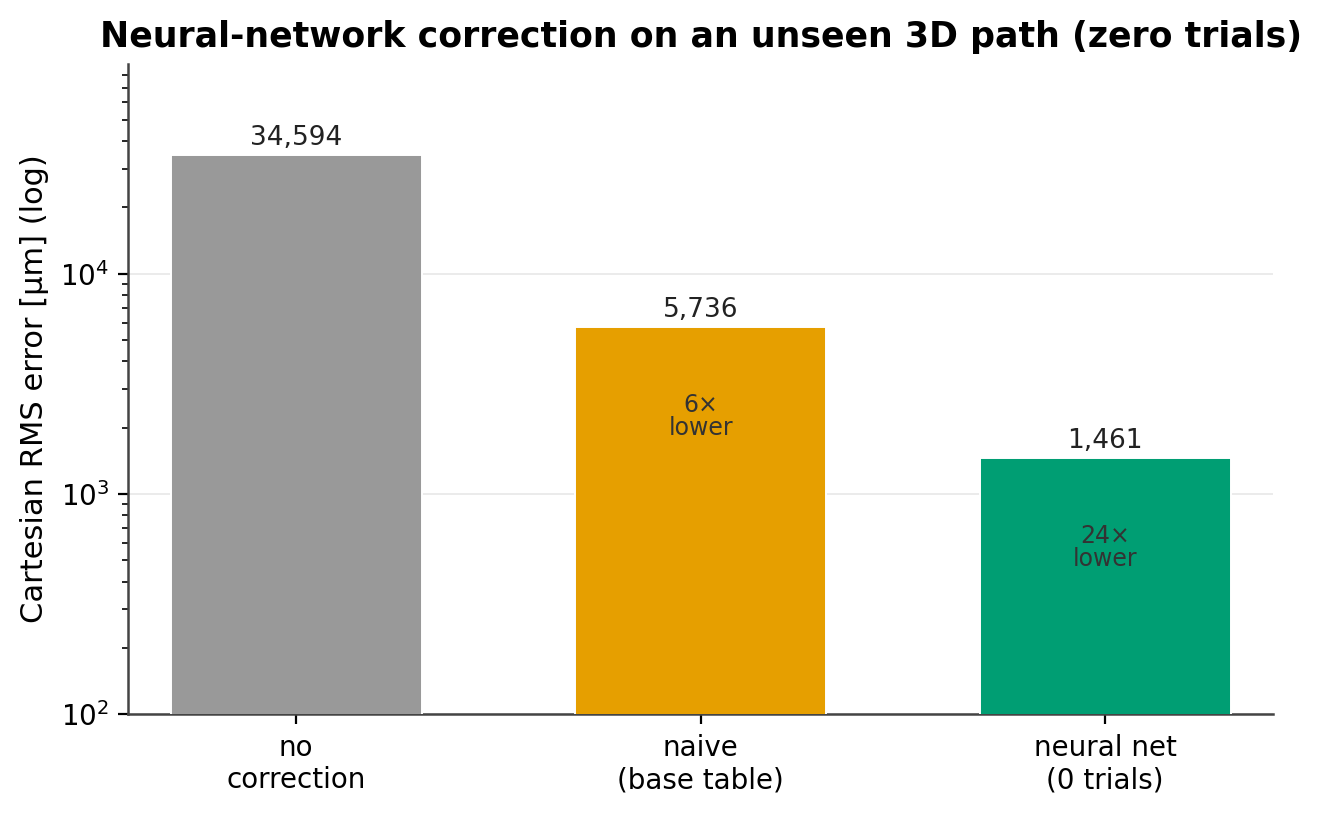
\includegraphics[width=\linewidth]{../outputs/kuka_nn_path_transfer.png}\\[0.3mm]
{\footnotesize\textbf{Unseen path}, 0 trials: 34594$\to$5736$\to$\num{1461\,$\mu$m}\\\why{instant vs.\ re-running ILC trials}}\end{minipage}\hfill
\begin{minipage}[t]{0.325\linewidth}\centering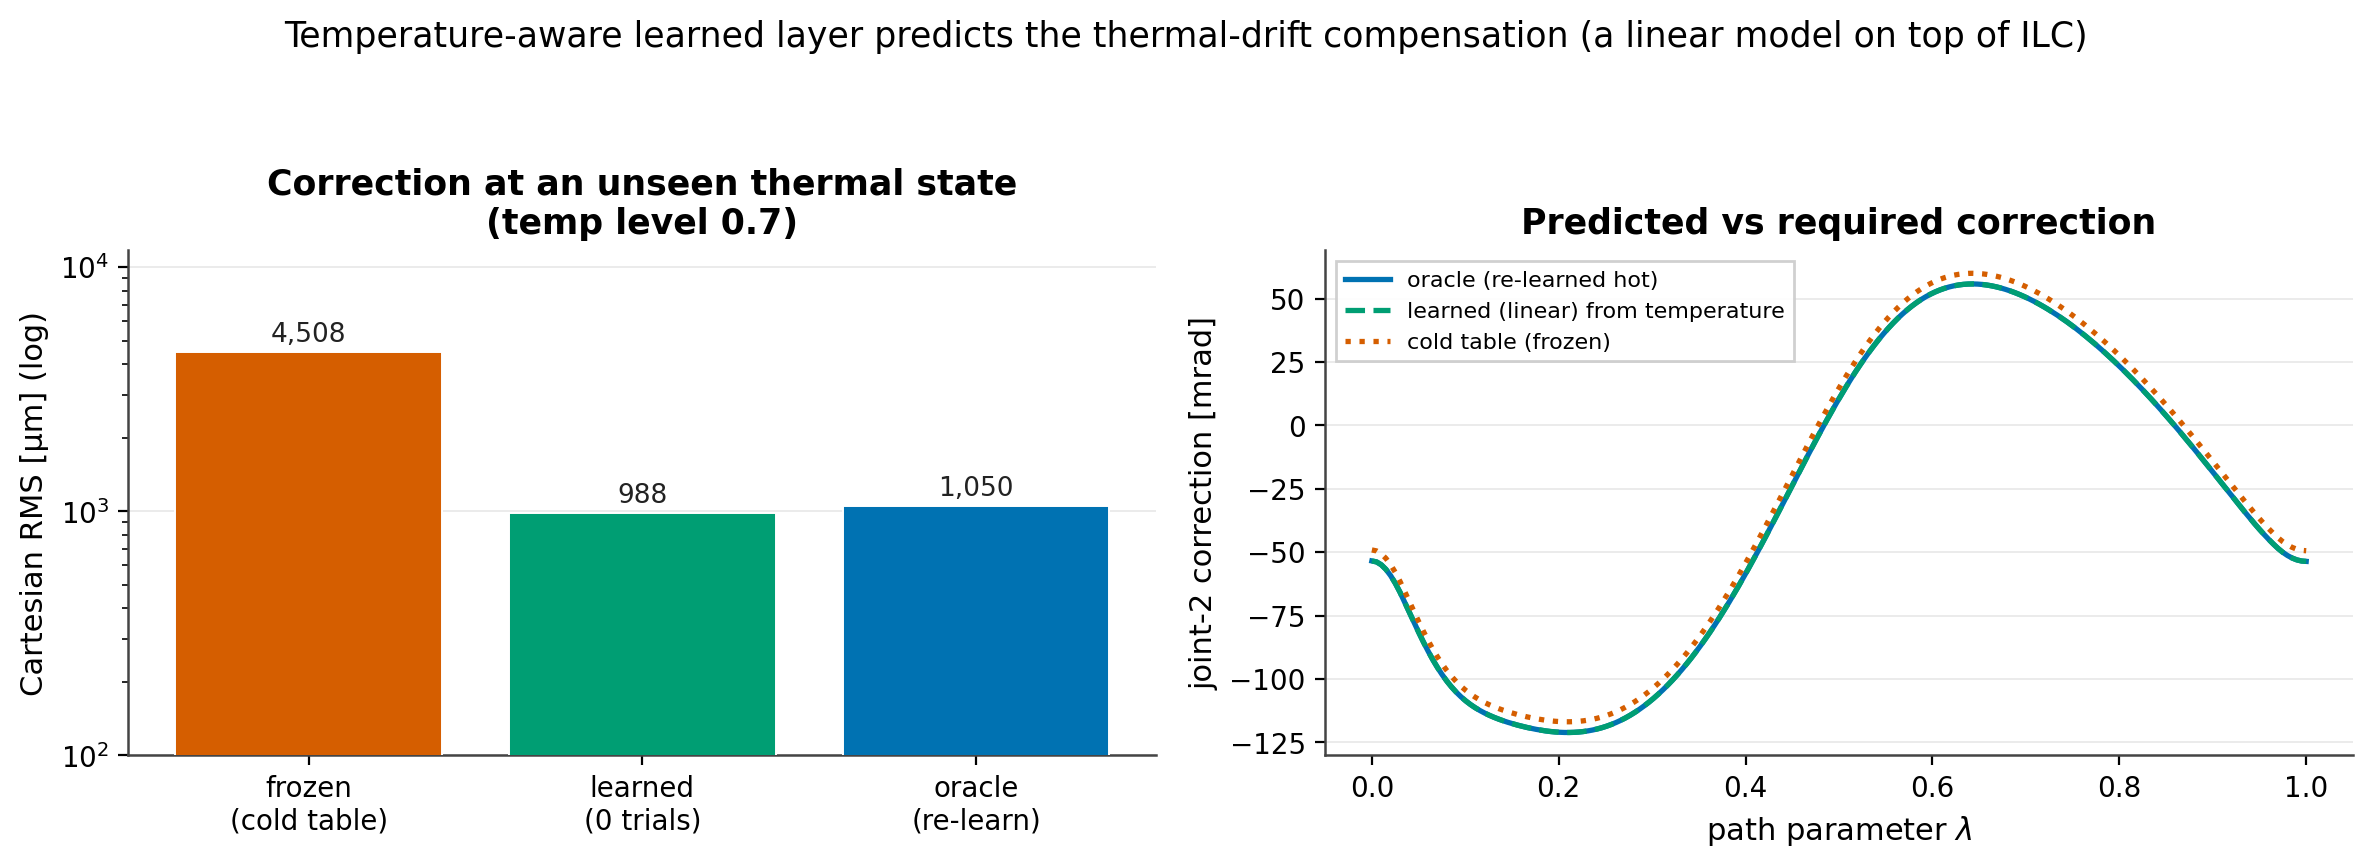
\includegraphics[width=\linewidth]{../outputs/thermal_learned_compensation.png}\\[0.3mm]
{\footnotesize\textbf{Unseen thermal state}: frozen 4508$\to$\num{988}$\approx$oracle 1050\,$\mu$m\\\why{a fixed table cannot track drift; this can}}\end{minipage}
\end{minipage}
\vspace{1.2mm}\rule{\linewidth}{0.4pt}\\[0.5mm]
{\footnotesize\textbf{Honest scope.} Simulation. The joint-side (output) encoder \emph{directly} observes the link, so learning-without-a-tracker here is a \emph{stronger} sensing assumption than the paper's motor-encoder-only robot; real secondary encoders have noise/resolution limits and a joint$\to$task kinematic-calibration gap remains. Speed transfer is partial. \textbf{Reproduce all figures:} \texttt{python src/run\_all.py}.}

% ===================== PAGE 2 : figure appendix =====================
\newpage
{\centering
{\LARGE\bfseries Appendix --- analysis (a--d) \& realistic-effects (e--i) figures}\\[0.8mm]
{\small Supporting evidence behind the headline results --- one panel per claim (cf.\ \texttt{FIGURES.md}). Cartesian RMS at the tool tip; simulation, seeded.}\\[1mm]}
\rule{\linewidth}{1pt}\\[2.5mm]
\appfig{trialwise_overview.png}{\textbf{(a)} --- paper Fig.\,5 reproduction: TCP error / ILC inputs / path speed over 7 trials (trial 5 ILC-\emph{off}, 6 \emph{on}).}\hfill
\appfig{encoder_validation.png}{\textbf{(b)} --- no-tracker validation: joint-side encoder RMS vs true TCP RMS in lock-step (corr 0.97).}\hfill
\appfig{error_along_path.png}{\textbf{(c)} --- where the error lives along the path, before vs after learning (log scale).}\\[3mm]
\appfig{joint_modal_properties.png}{\textbf{(d)} --- mechanical view: each joint a torsional spring-mass-damper; $f_n$ 10--195\,Hz vs the Q-filter cutoff.}\hfill
\appfig{realistic_effects_ablation.png}{\textbf{(e)} --- ablation: ILC stays $\sim$1\,mm under every realistic effect (repeatable learned, noise filtered).}\hfill
\appfig{qfilter_noise_rejection.png}{\textbf{(f)} --- the Gaussian Q-filter rejects encoder noise (the learned correction is jagged without it).}\\[3mm]
\appfig{transmission_error_profile.png}{\textbf{(g)} --- the injected angle-periodic transmission error (gear/cycloidal harmonics, 13--37 cyc/rev).}\hfill
\appfig{thermal_frozen_vs_online.png}{\textbf{(h)} --- thermal drift defeats a frozen ILC table; an online ILC tracks the warm-up.}\hfill
\appfig{thermal_learned_compensation.png}{\textbf{(i)} --- temperature-aware learned model predicts the thermal compensation at an \emph{unseen} state, 0 trials.}
\end{document}
